\chapter{Emergence of traveling waves in linear arrays of electromechanical oscillators$^{*}$}
\begin{center}
\vspace*{1\baselineskip}
\textbf{Abstract}
\end{center}
Traveling waves of mechanical actuation provide a versatile strategy for locomotion and transport in both natural and engineered systems across many scales. These rhythmic motor patterns are often orchestrated by systems of coupled oscillators such as beating cilia or firing neurons. Here, we show that similar motions can be realized within linear arrays of conductive particles that oscillate between biased electrodes through cycles of contact charging and electrostatic actuation. The repulsive interactions among the particles along with spatial gradients in their natural frequencies lead to phase-locked states characterized by gradients in the oscillation phase. The frequency and wavelength of these traveling waves can be specified independently by varying the applied voltage and the electrode separation. We demonstrate how traveling wave synchronization can enable the directed transport of material cargo. Our results suggest that simple energy inputs can coordinate complex motions with opportunities for soft robotics and colloidal machines.

%%%%%%%%%%%%%%%%%%%%%%%%%%%%%%%%%%%
%%%%%%%%%%%%%%%%%%%%%%%%%%%%%%%%%%%
%%%%%%%%%%%%%%%%%%%%%%%%%%%%%%%%%%%
\section{introduction} \footnotetext[1]{This chapter is adapted from  "Dou, Y., Pandey, S., Cartier, C. A., Miller, O., & Bishop, K. J. (2018). Emergence of traveling waves in linear arrays of electromechanical oscillators. \textit{Communications Physics}, 1(1), 1-9."}

Traveling waves of mechanical actuation provide a versatile strategy for locomotion and transport in both natural\autocite{Cohen1982, Blake1974, Taylor447, purcell1977life} and engineered\autocite{Palagi2016,Park2016} systems across many scales. In vertebrates such as the aquatic lamprey \autocite{Cohen1982, Cohen1992}, these and other rhythmic motor patterns are orchestrated by networks of neurons called central pattern generators (CPGs) \autocite{Marder2001}, which are often idealized as systems of coupled oscillators \autocite{Cohen1982, Cohen1992}. The rhythmic output of these oscillators is relayed to actuators (e.g., muscles) to produce complex motions without the need for sensory feedback. Similar control strategies based on CPGs are used to direct  locomotion in macroscopic robots \autocite{Ijspeert2008}. At smaller scales, however, it becomes increasingly challenging to accommodate centralized control systems capable of directing the coordinated actions of multiple actuators. Instead, microorganisms such as ciliated protozoa integrate pattern generation and mechanical actuation within a single material system.  The oscillatory motions of beating cilia couple to one another through hydrodynamic interactions to produce metachronal waves that drive cellular locomotion through viscous surroundings \autocite{Blake1974, Niedermayer2008, Elgeti2013}. This biological example illustrates how the coupled motions of many mechanical oscillators can organize spontaneously and autonomously to perform dynamic functions.}

The realization of synthetic systems that mimic such functions requires experimental strategies for powering mechanical oscillators and for coupling their motions to achieve the desired dynamics. One approach relies on coupling reaction-diffusion patterns to the mechanical deformation of responsive gels, for example, to achieve traveling wave motions in excitable media \autocite{Masuda2016}. Despite fascinating demonstrations of this approach on millimeter length scales, it remains challenging to miniaturize due to the need for faster reactions that compete with diffusion at smaller scales. To achieve scalable mechanisms of pattern formation, the processes that drive oscillations should scale in the same way as those used to couple neighboring oscillators. In this context, electromechanical oscillators based on contact charge electrophoresis (CCEP) \autocite{bishop2018contact,drews2015contact} can provide a useful model on length scales spanning millimeters\autocite{Mersch2011} to microns\autocite{Dou2016} (perhaps even nanometers \autocite{Park2000,Kowalik2016}).
CCEP refers to the back-and-forth motion of a conductive particle \resp{through an insulating fluid separating} two electrodes subject to a constant voltage. \resp{The particle charges on contact with either electrode and moves down the applied potential gradient, thereby transporting charge between the biased electrodes. This type of electromechanical oscillator is fundamentally distinct from the weakly damped harmonic oscillators of micro-electromechanical systems (MEMS)\autocite{van2011review,Zhang2014}, which rely on resonant excitation by time-varying fields. By contrast, CCEP oscillators are powered by a constant thermodynamic driving force and operate even under conditions of strong damping, which arise at small scales and in viscous environments.  Similar to those of molecular motors\autocite{Kolomeisky2007,Kowalik2016}, CCEP motions can be rectified to perform mechanical work or to transport material cargo\autocite{drews2013ratcheted,Kowalik2016}. Moreover,} the charge acquired by the particle and the forces driving its motion are well described by classical electrostatics, which is invariant to changes in scale. The discovery of new CCEP motions at the macroscale is therefore transferable to emerging applications at the microscale\autocite{bishop2018contact}.
Here, we investigate the collective dynamics of many CCEP oscillators positioned along a linear array between two (nearly) parallel electrodes (Fig.~\ref{fig:3.1}a). Each oscillator is comprised of a conductive sphere that moves back and forth between the electrodes along a dielectric track.  Oscillatory motions are driven by the repeated charging of the particles on contact with either electrode and their subsequent movement in the applied field. The dynamics of neighboring oscillators are coupled to one another through the electrostatic interactions between the charged particles. We show how this electrostatic coupling mediates the organization of phase-locked states in which all oscillators move with a common frequency. Interestingly, the distribution of oscillator phases at steady state corresponds to traveling waves of particle motion with a characteristic wavelength comparable to the electrode separation. These experimental observations are explained by a Kuramoto-like model\autocite{Acebron2005,Tsimring2005} that accounts for weak repulsive coupling between neighboring phase oscillators and for small systematic variations in their natural frequencies. We demonstrate how traveling wave synchronization can be used to transport material cargo along the length of the oscillator array. More generally, our approach shows how simple energy inputs can power complex patterns of mechanical actuation, which may be useful in powering the motions of soft robots\autocite{rus2015design, acome2018hydraulically} and colloidal machines\autocite{Snezhko2011,Yan2012, Martinez-Pedrero2015, goodrich2017using, Driscoll2017}.

%%%%%%%%%%%%%%%%%%%%%%%%%%%%%%%%%%%
\begin{figure}[p!]
    \centering
    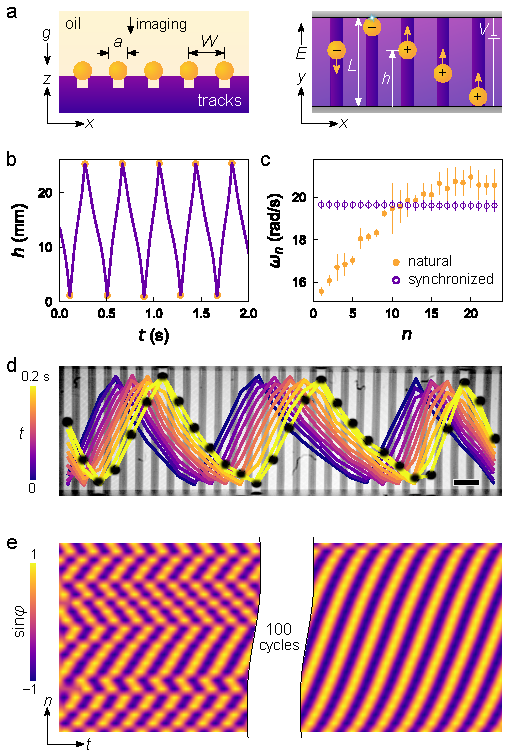
\includegraphics[width=10cm]{figures/3_1.pdf}
    \caption{Travelling wave synchronization. (a) Conductive spheres immersed in mineral oil oscillate along dielectric tracks connecting two plane electrodes subject to a constant voltage $V$. Particles charge on contact with each electrode and move in the electric field $E$. (b) Oscillatory dynamics of a single particle showing its position $h$  as a function of time $t$; yellow markers denote contacts with the electrodes. The applied voltage is $V=19$ kV; the electrode separation is $L=25$ mm. (c) Oscillation frequency $\omega_n$ as a function of the position $n$ along the array. The natural frequency of each oscillator varies with position (solid markers); all oscillators move with a common frequency in the synchronized state (open markers). Error bars represent the standard deviation in the instantaneous frequency, $2\pi/(t_{k+1}-t_k)$, over 100 cycles. (d) Image of the experiment showing particle positions at successive times; scale bar is 3 mm. (e) Space-time plot of the oscillator phase $\varphi$ showing the emergence of traveling wave synchronization for the $N=23$ oscillators in (c) starting from a random initial configuration.  Here, the track period is $W=3$ mm; other parameters are listed in (b).}
    \label{fig:3.1}
\end{figure}
%%%%%%%%%%%%%%%%%%%%%%%%%%%%%%%%%%%


%%%%%%%%%%%%%%%%%%%%%%%%%%%%%%%%%%%
%%%%%%%%%%%%%%%%%%%%%%%%%%%%%%%%%%%
%%%%%%%%%%%%%%%%%%%%%%%%%%%%%%%%%%%


\section{Results}

\subsection{Experiment}

Copper spheres ($a = 1$ mm in radius) immersed in mineral oil were positioned within an array of dielectric tracks connecting two plane electrodes separated by a distance $L$ (Fig.~\ref{fig:3.1}a). The tracks were spaced evenly with a period $W=3a$ and aligned perpendicular to the electrode surfaces and to the direction of gravity. Each track contained a single particle, which was free to move back and forth between the two electrodes. Application of a constant voltage (typically, $V=10$ kV) caused the particles to oscillate continuously between the electrodes via contact charge electrophoresis (CCEP) \autocite{bishop2018contact, drews2015contact}. The conductive particles acquired an electrostatic charge on contact with the biased electrodes and moved under the influence of the applied field. This periodic cycle of contact charging and electrostatic actuation continued for as long the voltage was applied.

% Dynamics of individual particles

%\noindent
%\textbf{Dynamics of electromechanical actuator arrays}
Figure \ref{fig:3.1}b shows the reconstructed trajectory of a single sphere oscillating between the two electrodes. Each time the particle contacts an electrode, its charge changes sign and the particle reverses direction under the influence of the field. To facilitate the analysis of multiple particles over many oscillation cycles, we record the times at which each particle contacts one of the electrodes.  From this data, we approximate the phase of each oscillator by interpolating between successive contacts as $\varphi(t) = 2\pi (t-t_k)/ (t_{k+1}-t_{k})$ where $t_k$ denotes the time of the $k^{th}$ contact and $t_k \leq t < t_{k+1}$. By definition, the oscillator phase increases at a constant rate equal to the natural frequency, $\mathrm{d}\varphi/\mathrm{d}t = \omega$, which is approximated by averaging over many oscillation cycles as $\omega = \langle 2\pi/(t_{k+1}-t_{k}) \rangle_k$. Repeating this analysis for each particle in isolation (i.e., one track at a time), we observed small systematic variations in the natural frequency $\omega_n$ with respect to the oscillator position $n$ along the array (Fig.~\ref{fig:3.1}c, solid markers). The spatial gradients in the oscillator frequency were caused by small deviations in the electrode alignment,  which was controlled only to within ca.~1$^\circ$ of parallel. Particles oscillated faster where the electrodes were closer together due to an increase in field strength at those locations.
        
% Dynamics of particle arrays
Despite variations in their natural frequencies, linear arrays of $N$ particle oscillators moving simultaneously evolved in time to a phase-locked state, in which each particle moved with a common frequency (Fig.~\ref{fig:3.1}c). Interestingly, the synchronized particles did not move in phase with one another but rather organized to form a single traveling wave, which remained stable for hundreds of oscillation cycles (Fig.~\ref{fig:3.1}d; Supplementary Movie 1). Space-time plots of the oscillator phase $\varphi_n(t)$ show how this wave-like pattern emerged from a disordered initial configuration (Fig.~\ref{fig:3.1}e; see also appendix. The direction of wave propagation was related to the spatial gradient in the oscillators' natural frequencies: waves traveled from slower to faster oscillators. Notably, the travelling wave patterns were robust to disturbances and recovered when disrupted by external perturbations (Supplementary Movie 3).

%%%%%%%%%%%%%%%%%%%%%%%%%%%%%%%%%%%
%%%%%%%%%%%%%%%%%%%%%%%%%%%%%%%%%%%
%%%%%%%%%%%%%%%%%%%%%%%%%%%%%%%%%%%

% The role of particle number $N$ 
The stability of the synchronized state and the distribution of oscillator phases therein depended on the number of oscillators $N$ in the array. For $N=2$ oscillators, the particles moved in antiphase as reported previously \autocite{Mersch2011} (Fig.~\ref{fig:3.2}a). Such antiphase synchronization suggests that neighboring oscillators are coupled together by repulsive interactions such as the Coulombic forces between like-charged particles. As the number of particles was increased, the average phase difference between successive oscillators decreased giving rise to stable traveling waves with wavelengths spanning many oscillators (Fig.~\ref{fig:3.2}b; see also Appendix). Beyond some critical number of oscillators $N^*$, the synchronized state became unstable (Fig.~\ref{fig:3.2}c). Above this threshold, traveling waves were observed to grow and break near the center of the array in a periodic fashion (Supplementary Movie 5). Such breaking events are characterized by dislocation-like defects in the space-time plots for the oscillator phases (Fig.~\ref{fig:3.2}c). The breaking frequency increased as the number of oscillators was increased beyond the stability threshold $N^*$ . For $N\gg N^*$, wave breaking was no longer periodic but rather occurred at irregular intervals and at different locations.
    
%%%%%%%%%%%%%%%%%%%%%%%%%%%%%%%%%%%
\begin{figure}[p!]
    \centering
    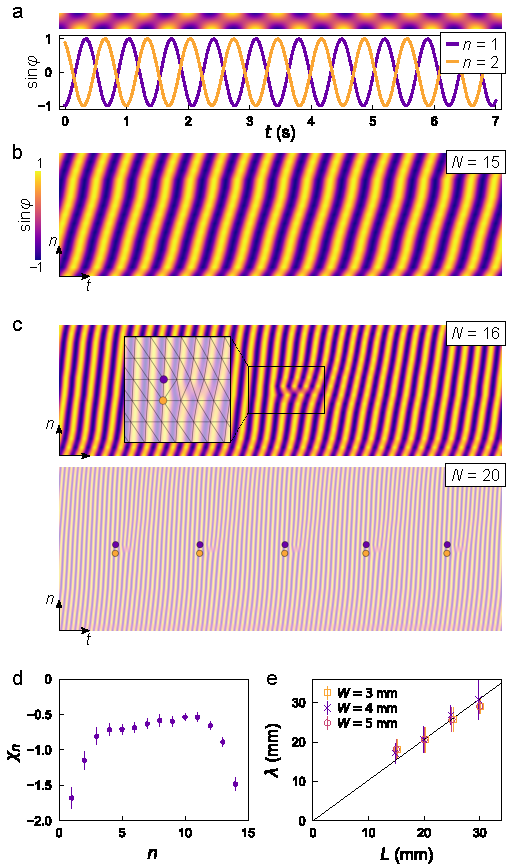
\includegraphics[width=10cm]{figures/3_2.pdf}
    \caption{Characterization of travelling waves (a) $N=2$ oscillators moving in antiphase. The plot shows the sine of the oscillator phases (bottom); the space-time image shows the same data in a different way (top). (b) Space-time plot for $N=N^*=15$ oscillators showing 20 oscillation cycles. (c) Space-time plots for $N>N^*$ showing defects that occur at regular time intervals. The markers show points in the space-time lattice with five-fold (purple) and seven-fold (yellow) coordination. (d) Time-averaged phase difference $\chi_n$ as a function of position $n$ for $N=N^*$ oscillators. Data for (a-d) were collected with $L=25$ mm, $W=3$ mm, and $V=18$ kV.  (e) Characteristic wavelength $\lambda$ as a function of the electrode separation $L$ for $N=N^*$ and different oscillator spacings $W$. Error bars represent the standard deviation from five independent experiments.}
    \label{fig:3.2}
\end{figure}
%%%%%%%%%%%%%%%%%%%%%%%%%%%%%%%%%%%

% Characteristic wavelength for $N=N^*$ (Fig.~\ref{fig:3})
To better understand the synchronized state, we quantified the distribution of oscillator phases for $N = N^*$ as a function of the electrode separation $L$ and the oscillator spacing $W$. For each electrode configuration, we started with $N>N^*$ oscillators and removed one particle at a time from the end of the array until reaching a stable synchronized state, at which the phase difference between neighboring oscillators was constant in time. Figure \ref{fig:3.2}d shows the time-averaged phase difference $\chi^{\s}_n = \langle \varphi_{n+1}(t) - \varphi_n(t) \rangle_t$ at the stationary state for a typical experiment. The phase difference was smallest (in magnitude) near the center of the array and largest near the edges. For each such state, we defined a characteristic wavelength in terms of the average phase difference as $\lambda = 2\pi W / \langle \chi_n^{\s} \rangle_n$. This wavelength increased linearly with the electrode spacing $L$ but was independent of the oscillator spacing $W$ over the range explored (Fig.~\ref{fig:3.2}e).

%%%%%%%%%%%%%%%%%%%%%%%%%%%%%%%%%%%%%%%
\subsection{Minimal Model of Traveling Wave Synchronization}

The experimental observations are reproduced by a Kuramoto-like model \autocite{Acebron2005} that accounts for the local repulsive coupling between neighboring oscillators and the systematic variations in their natural frequencies.  In the model, we adopt the following simplified description of CCEP dynamics\autocite{Kowalik2016}. \resp{On contact with either electrode, a conductive sphere acquires a charge $q = \pm \tfrac{2}{3}\pi^3\varepsilon a^2 E$, where $E$ is the electric field at the electrode surface, and $\varepsilon$ is the permittivity of the surrounding dielectric.  This expression---first derived by Maxwell\autocite{Maxwell1873}---assumes that charge flows to/from the particle until its potential equals to that of the contacting electrode\autocite{drews2014charge}. The electrostatic force on the particle is approximated as $F = q E$, which drives motion with velocity $U=F/\gamma$, where $\gamma$ is a constant friction coefficient. Figure \ref{fig:3.4}a shows how the charge $q$ and position $h$ of a single oscillator depend on its phase $\varphi=\omega_{\ro} t$, where $\omega_{\ro} = \pi q_{\ro} E_{\ro}/\gamma L$ is the natural frequency defined in terms of the applied field $E_{\ro}=V/L$ and the Maxwell charge $q_{\ro}=\tfrac{2}{3}\pi^3\varepsilon a^2 E_{\ro}$. By comparing the measured frequency in Fig.~\ref{fig:3.1}c to the prediction of the model, the friction coefficient can be estimated to be $\gamma=1.8\times10^{-3}$ N s m$^{-1}$, which ca.~4 times larger than the Stokes drag, $\gamma_{\text{s}}=6\pi\eta a$. The increased drag is attributed to the solid boundaries formed by the patterned tracks and the planar electrodes (Supplementary Fig.~5)\autocite{Goldman1967a}.}

% Interactions 
\resp{The presence of neighboring oscillators influences both the charge that a particle acquires and the speed at which it moves.  To describe these interactions, we decompose the electric field as $E=E_{\ro}+E'$, where $E_{\ro}$ is the applied field and $E'$ is a disturbance field due to neighboring particles, which are approximated as point charges (see Methods). In the limit of weak interactions (i.e., when $E'\ll E_{\ro}$), the moving particles are well approximated as phase oscillators with weak repulsive coupling between nearest neighbors.} The phase of the $n^{\text{th}}$ oscillator evolves in time as
\begin{equation}
    \frac{\partial \varphi_n}{\partial t} = \omega_n + f(\varphi_n - \varphi_{n-1}) + f(\varphi_n - \varphi_{n+1}), \label{eq:phase}
\end{equation}
where $\omega_n$ is the natural frequency, and the function $f(~)$ describes the phase-averaged interactions between neighboring oscillators as a function of their phase difference $\chi_n=\varphi_{n+1}-\varphi_n$. The boundaries of the array are open such that oscillators at the edges ($n=1,N$) interact with only one neighbor \autocite{Ottino-Loffler2016}. We assume a uniform gradient in the natural frequency:  $\omega_n = \omega_{\ro} +  \Delta \left[n-\tfrac{1}{2}(N+1)\right]$ for $n=1\dots N$, where $\omega_{\ro}$ is the mean oscillator frequency, and $\Delta$ is the frequency difference between successive oscillators due to a small angle $\theta$ between the electrodes ($\Delta/\omega_{\ro} \approx 3(W/L)\theta  \ll 1$).  Interestingly, this model was investigated previously as a possible explanation for traveling wave oscillations in the central pattern generator of the aquatic lamprey \autocite{Cohen1982}. 

%%%%%%%%%%%%%%%%%%%%%%%%%%%%%%%%%%%
\begin{figure}[p!]
    \centering
    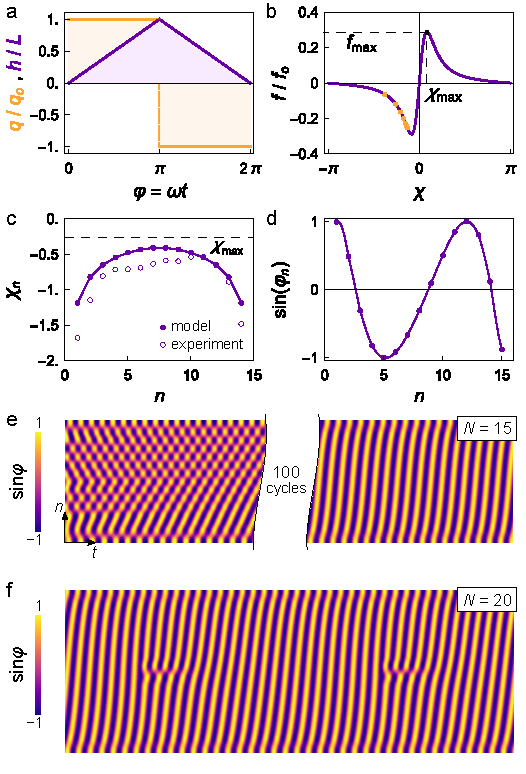
\includegraphics[width=10cm]{figures/3_3.pdf}
    \caption{Minimal model of traveling wave synchronization. (a) Charge $q$ and position $h$ of a idealized oscillator as a function of it phase $\varphi$. \resp{(b) Phase-averaged electrostatic interaction between two weakly-coupled oscillators as a function of their phase difference $\chi$. The interaction is scaled by $f_{\ro} = q_{\ro}^2/\varepsilon W^2 L \gamma$; the oscillator spacing is $W=0.12 L$. (c) Stable stationary solution for the phase difference $\chi_n$ of $N=15$ oscillators. Experimental data for the same conditions is reproduced for comparison. The predicted phase differences are plotted also in (b) to show their relationship with the interaction function $f(~)$. (d) Sine of the oscillator phase $\varphi_n$ showing the wave-like pattern.  (e) Dynamics of the $N=15$ oscillators starting from random initial conditions. (f) Oscillator dynamics for $N=20$ showing the periodic breaking of the traveling waves. In (c)--(e) the critical oscillator number is chosen to be $N^*=15.5$ as in experiment, which implies a frequency gradient $\Delta=0.0096 f_{\ro}$. The natural frequency is $\omega_{\ro}=\tfrac{3}{2\pi^2}(W/a)^2f_{\ro}=1.4 f_{\ro}$ where $W/a=3$ as in experiment; the ratio $\Delta/\omega_{\ro}=0.0070$ implies an electrode angle of $\theta=1.1^{\circ}$.}}
    \label{fig:3.4}
\end{figure}
%%%%%%%%%%%%%%%%%%%%%%%%%%%%%%%%%%%

% Description of the electrostatic interactions
In the present context, the primary interaction between neighboring oscillators is electrostatic in origin; other interactions are neglected. In particular, the neglect of hydrodynamic interactions was supported by experiments in which neighboring particles were separated by solid walls without altering their collective dynamics.  Approximating the particles as point charges, we compute the electrostatic interaction averaged over one oscillation cycle for a constant phase difference $\chi$ (see Methods). These repulsive interactions are described by an odd function characterized by the location $\chi_{\max}$ and height $f_{\max}$ of its maximum  (Fig.~\ref{fig:3.4}b).  For large electrode separations ($L\gg W$), these quantities are well approximated as $f_{\max}\approx \tfrac{1}{2\sqrt{3}} (q_{\ro}^2/\varepsilon W^2 L \gamma)$ and $\chi_{\max}\approx\tfrac{\pi}{\sqrt{2}} (W/L)$. \resp{Our assumption of weak coupling implies that the phase velocity due to interactions is small compared to the natural frequency---that is, $f_{\max}\ll\omega_{\ro}$ or, equivalently, $a/W\ll0.72$. Additional simulations incorporating the full amplitude dynamics provide further support for the phase oscillator approximation under the experimental conditions of $a/W=0.33$ (Supplementary Note 1 and Supplementary Fig.~7).}

% Stationary states of the minimal model
The competition between the repulsive interactions and the frequency gradient leads to stable stationary solutions described by $f(\chi_n) = -\frac{1}{2}\Delta n(N-n)$ (see Methods). This solution exists provided that the number of oscillators is below some critical value $N^* = \sqrt{8 f_{\max}/\lvert\Delta\rvert}$. Figure \ref{fig:3.4}c,d,e shows the stable solution in terms of the phase difference and the sine of the phase for $N=15$ oscillators---just below the chosen critical value of $N^*=15.5$. The addition of more particles ($N>N^*$) causes the waves to break periodically in the center of the array (Fig.~\ref{fig:3.4}f). Physically, faster oscillators pile up behind the slower ones and are prevented from passing by the local repulsive interactions.  In this way, the frequency gradient acts to compress the oscillator phases together to create longer waves that travel always from slower to faster oscillators. When compression by the frequency gradient exceeds the repulsive barriers between neighboring oscillators, global synchronization is lost and the waves break. 

At the critical oscillator number ($N = N^*$), repulsive interactions are at their maximum ($\chi^{\s}_n \sim \chi_{\max}$), and the characteristic wavelength scales linearly with the electrode separation in agreement with experimental observations (Fig.~\ref{fig:3.2}e)---that is, $\lambda\sim2\pi W/ \chi_{\max} \sim L$ for $W\ll L$.  Moreover, the critical oscillator number observed in experiment implies a certain angle between the electrodes, which can be estimated from the model as $\theta = \tfrac{1}{3}(L\Delta /W \omega_{\ro} ) = \tfrac{8 \pi ^2}{9 \sqrt{3}} (a^2 L/W^3 {N^*}^2)$. For the conditions of Figure \ref{fig:3.2}, this angle is predicted to be $\theta = 1.1^\circ$, which agrees well with that measured from the experimental images (Fig.~\ref{fig:3.1}b).  Smaller angles allow for stable waves containing more particles. 

The average phase within the wave evolves in time at a constant rate equal to the average frequency $\omega_{\ro}$, which is specified independently of the wavelength. In experiment, the oscillator frequency could be altered by changing the applied voltage; however, the range of accessible frequencies was limited by dielectric breakdown at higher voltages and by particle sticking at lower voltages\autocite{drews2015contact}. Notably, the frequency of the phase locked state was slightly faster than the average natural frequency (Fig.~\ref{fig:3.1}d). Dipolar interactions among the particles (neglected here) break the odd symmetry of the interaction function thereby altering the frequency of the synchronized state.


%%%%%%%%%%%%%%%%%%%%%%%%%%%%%%%%%%%
%%%%%%%%%%%%%%%%%%%%%%%%%%%%%%%%%%%
%%%%%%%%%%%%%%%%%%%%%%%%%%%%%%%%%%%
\section{Discussion}

We have shown how arrays of electromechanical oscillators can organize spontaneously to form synchronized traveling waves of particle motion powered by a constant input voltage.  The direction of wave propagation is determined by small gradients in the natural frequencies of the oscillators and can be controlled by introducing a small angle between the otherwise parallel electrodes.  The characteristic wavelength is approximately equal to the electrode separation $L$ and corresponds to the largest possible wave that can be stabilized by repulsive interactions among the charged particles.  The traveling wave motions are robust to perturbations and can be harnessed to direct the transport of material cargo.  In particular, Figure \ref{fig:3.5}a shows how traveling waves can direct the motion of gas bubbles floating at the interface just above the oscillating particles (see also Supplementary Movie 6).  Bubbles are transported in the direction of wave propagation at speeds comparable to the wave velocity (Fig.~\ref{fig:3.5}b). In contrast to previous strategies for rectifying CCEP motions based on ratcheted channels\autocite{drews2013ratcheted} or asymmetric particles\autocite{Dou2016}, the present approach relies on the self-organization of multiple particles working in concert. 

%%%%%%%%%%%%%%%%%%%%%%%%%%%%%%%%%%%
\begin{figure}[h]
    \centering
    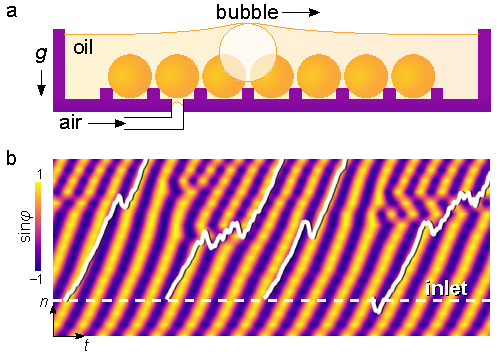
\includegraphics[width=10cm]{figures/3_4.pdf}
    \caption{Transport of air bubbles via travelling waves. (a) Schematic illustration of the experimental set-up from the side. (b) Trajectories of four bubbles (white) superimposed over the space-time plot of the oscillator phase. See also Supplementary Movie 6.}
    \label{fig:3.5}
\end{figure}
%%%%%%%%%%%%%%%%%%%%%%%%%%%%%%%%%%%
Beyond this initial demonstration, traveling wave synchronization of CCEP oscillators may be useful for peristaltic pumping within microfluidic systems. Unlike standard pressure pumps, those based on traveling wave motions allow for recirculating flows\autocite{mi5020289} and would complement existing  applications of CCEP in microfluidic cargo transport\autocite{drews2013ratcheted,cartier2017electric}, separations\autocite{drews2013ratcheted}, and fluid mixing\autocite{cartier2014microfluidic}. These CCEP-powered unit operations rely on constant voltages at low input power, which makes them attractive for use in portable, battery-powered microfluidic devices\autocite{bishop2018contact}.  One important limitation of these oscillators is their reliance on the dielectric environment provided by non-polar fluids; CCEP motions cannot be sustained in even weakly conductive liquids such as deionized water\autocite{cartier2014microfluidic}. However, recent advances in soft robotics suggest one strategy for circumventing this limitation by encapsulating non-polar liquids in stretchable, impermeable compartments\autocite{acome2018hydraulically}. These soft composite materials can be deformed by applying voltages to stretchable electrodes patterned on their surfaces.  By incorporating arrays of CCEP oscillators within such dielectric compartments, it should be possible to create self-organized motions that drive transient deformations and thereby locomotion of soft robotic materials.
\section{Methods}

%%%%%%%%%%%%%%%%%%%%%%%%%%%%%%%%%%%
\subsection{Experiment Set-up.} 
Periodic arrays of dielectric tracks were 3D printed in acrylonitrile butadiene styrene (ABS) with a period of $W=3-5$ mm. The array was sandwiched between two copper plates separated by a distance $L=10-30$ mm (McMaster-Carr 3350K201) and immersed in mineral oil (Sigma Aldrich CAS No.~8042-47-5). The tracks were aligned perpendicular to the electrode surfaces and to the direction of gravity. Each track contained a single copper sphere (McMaster-Carr No.~64715K16, radius $a=1$ mm), which rolled freely between the two electrodes (Fig.~\ref{fig:3.1}a). Prior to use, the system was heated in a 60$^\text{o}$C oven for several hours to remove any moisture. The copper electrodes were connected to a amplifier (Trek 20/20C) with an output voltage $V=0-20$ kV.  The particles were illuminated from below by a light emitting diode (LED) and their motions captured by a high-speed camera (Phantom V310).  During each experiment, the electrodes were energized to a specified voltage and the resulting particle motions captured. The voltage was switched off for at least one minute between successive experiments to allow for the dissipation of any space charge accumulated on the surfaces of the tracks and/or the electrodes.  Particle location data were extracted using standard image tracking routines in MATLAB.


%%%%%%%%%%%%%%%%%%%%%%%%%%%%%%%%%%%


%%%%%%%%%%%%%%%%%%%%%%%%%%%%%
\subsection{Electrostatic Interactions.}
We first consider a single point charge $q$ positioned at a height $z=h$ between two grounded planes at $z=0$ and $z=L$.  The resulting electrostatic potential at point $\ve{x}$ is 
\begin{equation}
    \phi(\ve{x}) = \frac{q}{\pi L \varepsilon} \sum_{m=1}^{\infty} \sin\left(\frac{m\pi h}{L}\right)  \sin\left(\frac{m\pi z}{L}\right) K_0\left(\frac{m \pi r}{L}\right),\label{eq:point}
\end{equation}
where $r=\sqrt{x^2 + y^2}$ is the radial distance from the charge, and $K_0(~)$ is the zeroth order modified Bessel function of the second kind. For large arguments, the Bessel function decays exponentially as $K_0(s)\rightarrow e^{-s}\sqrt{\pi/2 s} $; the infinite series can be truncated for some $m\gg L/\pi r$ to obtain an accurate approximation.  The corresponding electric field in the $z$-direction is given by $E_z = -\partial \phi / \partial z$. 

\resp{We now consider how the disturbance field $E'$ due to one oscillator $i$ influences the dynamics of another oscillator $j$ in the limit of weak coupling. At zeroth order in $E'$, the phase of each oscillator increases at a constant rate $\omega_{\ro}$ such that $\varphi_i=\omega_{\ro} t$ and $\varphi_j=\omega_{\ro} t+\chi$, where $\chi=\varphi_j-\varphi_i$ is the constant phase difference.  The charge $q=q(\varphi)$ and position $h=h(\varphi)$ of each oscillator depends on the phase as shown in Figure~\ref{fig:3.4}a. At first order in $E'$, the disturbance in the phase of oscillator $j$ evolves as
\begin{equation}
    \frac{d \varphi'_j}{d t} = \frac{\pi n(\varphi_j)}{L\gamma} \left[q(\varphi_j) E'(\varphi_i,\varphi_j) + q'(\varphi_i,\varphi_j) E_{\ro} +\dots\right], \label{eq:j}
\end{equation}
where the factor $\pi n(\varphi_j)/L\gamma$ relates the electric force to the corresponding phase velocity with $n(\varphi_j)=\pm 1$ indicating the direction of travel. The bracketed terms describe two types of electrostatic interactions. First, the disturbance field due to particle $i$ drives particle $j$ to move faster or slower between the electrodes. Using the point charge solution (\ref{eq:point}), this disturbance $E'(\varphi_i,\varphi_j)$ is given by
\begin{equation}
    E'(\varphi_i,\varphi_j) = -\frac{q(\varphi_i)}{L^2 \varepsilon} \sum_{m=1}^{\infty} m \sin\left(\frac{m\pi h(\varphi_i)}{L}\right)  \cos\left(\frac{m\pi h(\varphi_j)}{L}\right) K_0\left(\frac{m \pi W}{L}\right),
\end{equation}
where $W$ is the oscillator spacing. Second, the disturbance field due to particle $i$ alters the charge acquired by particle $j$ on contact with either electrode; the disturbance charge $q'(\varphi_i,\varphi_j)$ is given by 
\begin{equation}
    q'(\varphi_i,\varphi_j) = \begin{cases} 
    +\tfrac{2}{3}\pi^3 \varepsilon a^2  E'(-\chi,0) & 0 \leq \varphi_j < \pi
    \\
    -\tfrac{2}{3}\pi^3 \varepsilon a^2 E'(\pi-\chi,\pi) & \pi \leq \varphi_j < 2\pi
    \end{cases}.
\end{equation}
Physically, the charge on particle $j$ is determined by its most recent contact with either electrode ($\varphi_j=0$ or $\pi$); the field due to particle $i$ at the time of that contact determines the disturbance charge.}

We can now average these two interactions over one oscillation cycle to obtain the phase-averaged interaction function,
\begin{equation}
    f(\chi) = \frac{\pi}{L\gamma}\frac{1}{2 \pi}\int_0^{2\pi} n(\varphi_j) \left[ q(\varphi_j) E'(\varphi_j-\chi,\varphi_j) + q'(\varphi_j-\chi,\varphi_j) E_{\ro} \right] d\varphi_j.
\end{equation}
Carrying out the integration, each of the two electrostatic interactions produce contributions of the same mathematical form with the second term contributing twice that of the first,
\begin{equation}
     f(\chi) = \frac{3\pi q_{\ro}^2}{2  \varepsilon L^3\gamma} \sum_{m=1}^{\infty} m \sin(m \chi)  K_0\left(\frac{m\pi W}{L}\right).
\end{equation}
This final expression is plotted in Figure \ref{fig:3.4}b for the case of $W/L=0.12$.


%%%%%%%%%%%%%%%%%%%%%%%%%%%%%%%%%%%
\subsection{Stationary Solution.} 
Starting from Eq.~(\ref{eq:phase}), we recast the oscillator dynamics in terms of the phase difference $\chi_n=\varphi_{n+1} - \varphi_n$ and the average phase $\Phi=\tfrac{1}{N}\sum_n\varphi_n$.  Taking the difference in the phase dynamics of successive oscillators, we obtain the following equation for the phase difference 
\begin{equation}
    \frac{\partial \chi_n}{\partial t} = \Delta - f(\chi_{n-1}) + 2 f(\chi_n) - f(\chi_{n+1})\quad\text{for }n=2,\dots,N-2, \label{eq:diff}
\end{equation}
which makes use of the fact that $f(~)$ is an odd function.  At the open boundaries of the array, the phase difference evolves as
\begin{equation}
    \frac{\partial \chi_1}{\partial t} = \Delta + 2f(\chi_1) - f(\chi_2)\quad\text{and}\quad\frac{\partial \chi_{N-1}}{\partial t} = \Delta - f(\chi_{N-2}) + 2f(\chi_{N-1}). \label{eq:diffBC}
\end{equation}
In addition to these $N-1$ equations, the dynamics of the $N$ oscillators is described by the that of the average phase, $\partial \Phi /\partial t = \omega_{\ro}$, which is fully decoupled from the phase differences. Setting the time derivatives in Eqs.~(\ref{eq:diff}) and (\ref{eq:diffBC}) equal to zero, the resulting recurrence equation can be solved to obtain the stationary solution, $f(\chi_n) = \tfrac{1}{2}\Delta n(n-N)$, presented in the main text. This solution exists provided that $f_{\max}>\tfrac{1}{8}N^2\lvert\Delta\rvert$ (Supplementary Note 2) and is stable when $f'(\chi_n)<0$ (Supplementary Note 3). The characteristic relaxation time for approaching the stationary state is given by the diffusive-like scaling relation $\tau\sim \chi_{\max}N^2/\pi^2 f_{\max}$.


%%%%%%%%%%%%%%%%%%%%%%%%%%%%%%%%%%%
%%%%%%%%%%%%%%%%%%%%%%%%%%%%%%%%%%%
